\documentclass{beamer}

\mode<presentation>
{
	\usetheme[
		titlepagelogo=logo_verticale_BLACK.png,% Logo for the first page
		language=italian,
		coding=utf8,
		bullet=square,
		pageofpages=di,
		color=blue,
		secondsupervisor=true,
	]{TorinoTh}
	
}

\usepackage[italian]{babel}
\usepackage{mathtools}

\def\spacedmiddle#1{\mathrel{}\middle#1\mathrel{}}

\title
{Macchine di Turing Quantistiche}

\author
{Pietro Zignaigo}

\institute
{Università di Genova}

\rel
{Elena Zucca}
\secondsupervisor
{Francesco Dagnino}

\date
{16-12-2024}

\subject
{Macchine di Turing Quantistiche}
% This is only inserted into the PDF information catalog. Can be left
% out.


% If you wish to uncover everything in a step-wise fashion, uncomment
% the following command: 

%\beamerdefaultoverlayspecification{<+->}


\begin{document}

\begin{frame}
	\titlepage
\end{frame}

\begin{frame}
	\tableofcontents
\end{frame}

\section{Introduzione}

\subsection{Computazione quantistica}

\begin{frame}{\subsecname}{}
	\begin{itemize}
		\item \textbf{Quantum advantage}: A parità di problema, la complessità temporale degli algoritmi quantistici può essere minore di quella degli algoritmi classici.
		\item Lo stato di un computer quantistico è una sovrapposizione di stati discreti.
	\end{itemize}
\end{frame}

\begin{frame}{\subsecname}{Spazi di Hilbert}
	\begin{itemize}
		\item Per modellare uno stato quantistico si utilizzano gli \textit{spazi di Hilbert}:
	\end{itemize}
	\[ \ell^{2} \left ( \mathcal{B} \right ) = \left \{ \phi : \mathcal{B} \rightarrow \mathbb{C} \spacedmiddle | \sum_{\mathcal{C} \in \mathcal{B}} \left | \phi \left ( \mathcal{C} \right ) \right |^{2} < \infty \right \}\]
	\begin{itemize}
		\item Per ragioni fisiche, possono essere applicati agli elementi dello spazio solo \textit{operatori unitari}:
		\begin{itemize}
			\item invertibili
			\item conservano la norma
		\end{itemize}
	\end{itemize}
\end{frame}

\subsection{Macchina di Turing}

\begin{frame}{\subsecname}{}
	\centering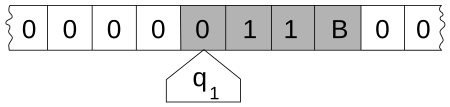
\includegraphics[width=6.5cm]{Turing_machine_2b.svg.png}
	\begin{itemize}
		\item Modello matematico per una macchina che esegue un certo algoritmo.
		\item \textbf{Funzioni calcolabili}: Funzioni parziali \( f : \mathbb{N} \rightarrow \mathbb{N} \) che sono calcolabili da una macchina di Turing.
	\end{itemize}
\end{frame}

\section{Macchina di Turing Quantistica}

\subsection{Configurazioni}

\begin{frame}{\subsecname}{}
	\begin{itemize}
		\item Una configurazione, ovvero lo stato di una macchina di Turing, è una quadrupla:
		\[ \left \langle \alpha, q, \beta, i \right \rangle \in \Sigma^{*} \times \mathcal{Q} \times \Sigma^{*} \times \mathbb{Z} \]
		\item \textbf{Q-configurazioni}: Elementi di \( \ell^{2}_{1} \left ( \Sigma^{*} \times \mathcal{Q} \times \Sigma^{*} \times \mathbb{Z} \right ) \).
	\end{itemize}
\end{frame}

\begin{frame}{\subsecname}{Contatore}
	\begin{itemize}
		\item Come mantenere inalterato il risultato dopo il raggiungimento di uno stato finale?
		\item Soluzione: aggiungere un contatore, la configurazione diventa:
		\[ \left \langle \alpha, q, \beta, i, n \right \rangle \in \Sigma^{*} \times \mathcal{Q} \times \Sigma^{*} \times \mathbb{Z} \times \mathbb{N} \]
		Chiamiamo questo insieme \(\mathfrak{C}_M\).
		\item Le q-configurazioni diventano elementi di: \( \ell^{2}_{1} \left ( \mathfrak{C}_M \right ) \).
	\end{itemize}
\end{frame}

\subsection{Funzione \texorpdfstring{\(\delta\)}{δ}}

\begin{frame}{\subsecname}{}
	\begin{itemize}
		\item
	\end{itemize}
\end{frame}

\subsection{Macchina di Turing Quantistica}

\begin{frame}{\subsecname}{}
	\begin{itemize}
		\item
	\end{itemize}
\end{frame}

\subsection{Unitarietà}

\begin{frame}{\subsecname}{}
	\begin{itemize}
		\item Perché l'operatore, visto in forma matriciale, sia unitario:
		\begin{enumerate}
			\item Deve avere le colonne con norma 1 (perché la norma sia sempre conservata)
			\item Ogni coppia di colonne deve essere ortogonale, ovvero due configurazioni pure non possono sovrapporsi dopo aver applicato l'operatore
		\end{enumerate}
		\item Esiste un teorema che garantisce l'unitarietà se \(\delta\) rispetta certe condizioni.
	\end{itemize}
\end{frame}

\section{Funzioni calcolabili quantistiche}

\subsection{Definizione}

\begin{frame}{\secname}{}
	\begin{itemize}
		\item Una \textit{Partial Probability Distribution (PPD)} è una funzione \( \mathcal{P} : \mathbb{N} \rightarrow \mathbb{R}_{[0,1]} \) tale che \( \sum_{n \in \mathbb{N}} \mathcal{P} \left ( n \right ) \le 1 \)
		\item \textbf{Funzioni calcolabili quantistiche}: Funzioni \( f : \ell^{2}_{1} \left ( \mathbb{N} \right ) \rightarrow PPD \) che sono calcolabili da una Macchina di Turing Quantistica.
	\end{itemize}
\end{frame}

\subsection{Categorie di terminazione}

\begin{frame}{\subsecname}{}
	\begin{enumerate}
		\item
	\end{enumerate}
\end{frame}

\section{Misurazioni}

\begin{frame}{\secname}{}
	\begin{itemize}
		\item
	\end{itemize}
\end{frame}

\end{document}